\documentclass[xcolor=table, aspectratio=169, bigger]{beamer}

\usepackage{shyne}

% Theme settings
\setbeamertemplate{navigation symbols}{}

\usetheme{Madrid}
\usefonttheme{structurebold}
\usefonttheme[onlymath]{serif}

\AtBeginSection[]
{ 	\begin{frame}{}

	{
	\usebeamerfont{frametitle}
	\begin{beamercolorbox}
		[wd={\textwidth}, center, sep=.2in, rounded=true, shadow=true]
		{frametitle}
	Week \thesection\\  \secname 
	\end{beamercolorbox}
	}
	
	\end{frame} 
}

\AtBeginSubsection[]
{ 	\begin{frame}{}

	{
	\usebeamerfont{frametitle}
	\begin{beamercolorbox}
		[wd={\textwidth}, center, sep=.2in, rounded=true, shadow=true]
		{frametitle}
	Section \thesection .\thesubsection\\  \subsecname 
	\end{beamercolorbox}
	}
	
	\end{frame} 
}

\title[Week 2]{Stat 201: Statistics I\\ Week 2}
\author[M. Shyne]{}
\institute[Metro State]{
\includegraphics[width=1.75in]{../images/metro_logo}}
\date[12/9/2018]{
\\ \bigskip \bigskip 
\includegraphics[width=.4in]{../images/cc_big}}


\begin{document}
\frame{\titlepage}

%
% Week 2
%
\setcounter{section}{1}
\section{Introduction to Probability}

%
% Section 2.1
%
\subsection{Basic Concepts of Probability}

\begin{frame}{Terms}
\begin{block}{}
A \bt{trial} is conducted to obtain a result from a process with uncertain outcomes. Also can be referred to as a random \bt{procedure} or \bt{process}.
\end{block}

\pause

\begin{block}{}
An \bt{event} is an outcome of interest from a trial.
\end{block}

\pause

\begin{block}{}
A \bt{simple event} is an event that cannot be broken down into simpler parts.
\end{block}

\pause

\begin{block}{}
A \bt{sample space} is the set of all possible simple events for a trial.
\end{block}
\end{frame}

%%%%%%%%%%
\begin{frame}{Terms, example}
\begin{exampleblock}{Example}
Consider flipping a coin...
\pause
\begin{itemize}
\item \bt{Trial:} \pause One flip of a coin
\pause
\item \bt{Event:} \pause Getting heads (H)
\pause
\item \bt{Simple event:} \pause This event cannot be broken down, it is a simple event
\pause
\item \bt{Sample space:} \pause Two possible events: \{ H, T \}
\end{itemize}
\end{exampleblock}
\end{frame}

%%%%%%%%%%
\begin{frame}{Terms, example cont.}
\begin{exampleblock}{Example}
Consider flipping a coin three times...
\begin{itemize}
\pause
\item \bt{Trial:} \pause Three flips of a coin
\pause
\item \bt{Event:} \pause Getting two heads and a tail
\pause
\item \bt{Simple event:} \pause There are several ways this event can occur. It can be broken down into \{ HHT, HTH, THH \}. Getting heads on the first two flips and tails on the third (HHT) is a simple event.
\pause
\item \bt{Sample space:} \pause Eight possible simple events:\\ \{ HHH, HHT, HTH, HTT, THH, THT, TTH, TTT \}
\end{itemize}
\end{exampleblock}

\end{frame}

%%%%%%%%%%
\begin{frame}{Probability}
\begin{block}{}
\bt{Probability} is a measure of the chance an event will occur in a trial.
\begin{itemize}
\pause
\item Though sometimes expressed as a percentage, probability is always a number between 0 and 1. 
\pause
\item Probability of 1 means the event is certain to occur and probability of 0 means it is impossible.
\end{itemize}
\end{block}
\pause
\begin{block}{}
Can interpret probability in two ways:
\begin{itemize}
\pause
\item Probability is the proportion an event will occur over a large number of trials. The \bt{law of large numbers} says this proportion will approach the ``true" probability as the number of trials increases.

\pause
\item Some trials can't be repeated (i.e. the weather tomorrow). Then, probability is the level of confidence that an event will occur in a trial (30\% chance of rain tomorrow). 
\end{itemize}
\end{block}
\end{frame}

%%%%%%%%%%
\begin{frame}{Notation}
\begin{block}{}
Events are designated with capital letters:
\pause
\begin{itemize}
\item $A$ = Get two heads and a tail in three coin flips
\item $B$ = Rain tomorrow
\item $C$ = A randomly selected person is taller than 78 inches
\end{itemize}
\end{block}

\pause
\begin{block}{}
Probabilities are designated with $P()$.
\pause
\begin{itemize}
\item $P(A)$ is the probability of event $A$.
\end{itemize}
\end{block}
\end{frame}

%%%%%%%%%%
\begin{frame}{Determining probabilities}
\begin{block}{}
\bt{Classical Approach:} If all simple events are equally likely, then\\
\medskip
\eq{P(A) = \frac{\text{number of simple events satisfying } A}{\text{total number of simple events in sample space}}}
\end{block}

\pause

\begin{block}{}
\bt{Relative Frequency Approximation:} Given a sample of trials,\\
\medskip
\eq{P(A) = \frac{\text{number of times } A \text{ occured}}{\text{number of trials}}} 
\end{block}

\end{frame}

%%%%%%%%%%
\begin{frame}{Classical approach, example}
\begin{exampleblock}{Example}
Consider flipping a coin three times. Assuming a fair coin, all simple events are equally likely. Recall the sample space,\\
\smallskip
{\centering
\{ HHH, HHT, HTH, HTT, THH, THT, TTH, TTT \} \par
}
\begin{itemize}
\pause
\item $A$ = Get two heads and a tail, \{ HHT, HTH, THH \}
\pause
\\\eq{P(A) = \frac 3 8}

\pause
\item $B$ = Get \emph{at least} two heads,  \{ HHH,  HHT, HTH, THH \}
\pause
\\\eq{ P(B) = \frac 4 8 = \frac 1 2}
\end{itemize}
\end{exampleblock}
\end{frame}

%%%%%%%%%%
\begin{frame}{Relative frequency, example}

\begin{exampleblock}{Example}
The Youth Risk Behavior Survey (YRBS) for 2015 reports that 9421 out of 15624 teenagers surveyed had driven a car at least once in the previous month. Of the 9421 teen drivers, 3806 had texted or emailed while driving. \\
\medskip
What is the probability that a randomly selected teen driver had texted or emailed while driving? 

\pause
\begin{itemize}
\item $A$ = Teen driver has texted or emailed while driving\\
\smallskip
\eq{P(A) = \frac {3806}{9421} = 0.404}
\end{itemize}

\end{exampleblock}

\end{frame}


%%%%%%%%%%
\begin{frame}{Complements}
\begin{block}{}
The \bt{complement} of event $A$, denoted as $\bar A$, consists of all outcomes in the sample space which are not included in $A$.
\begin{itemize}
\item Sometimes I'll call the complement of A simply ``not A.''
\end{itemize}
\end{block}

\pause
\begin{exampleblock}{Example}
\begin{itemize}
\item $A$ = Get a head on one coin flip\\
\pause
$\bar A$ = Get a tail on one coin flip

\pause
\item $B$ = Get exactly two heads on three coin flips\\
\pause
$\bar B$ = Get zero, one or three heads on three coin flips
\end{itemize}
\end{exampleblock}
\end{frame}
 
%%%%%%%%%%
\begin{frame}{Complement rule }
\begin{block}{}
Since an event and its complement ($A$ and $\bar A$) comprise all possible outcomes, then it is \emph{always} the case that\\
\eq{P(A) + P(\bar A) = 1}
\end{block}

\pause

\begin{exampleblock}{Example}
\begin{itemize}
\item One coin flip: $A$ = \{ H \}, $\bar A$ = \{ T \}\\
\pause
\eq{P(A) + P(\bar A) = \frac 1 2 + \frac 1 2 = 1}

\pause
\item Two heads in three coin flips: $B$ = \{ HHT, HTH, THH \},\\ $\bar B$ = \{ TTT, HTT, THT, TTH, HHH \}\\
\pause
\eq{P(B) + P(\bar B) = \frac 3 8 + \frac 5 8 = 1}
\end{itemize}
\end{exampleblock}
\end{frame}

%%%%%%%%%%
\begin{frame}{Using the complement rule}
\begin{exampleblock}{}
The Youth Risk Behavior Survey (YRBS) for 2015 reports that 9421 out of 15624 teenagers surveyed had driven a car at least once in the previous month. Of the 9421 teen drivers, 3806 had texted or emailed while driving. \\
\medskip
What is the probability that a randomly selected teen driver had \emph{not} texted or emailed while driving? 

\begin{itemize}
\pause
\item $A$ = Teen driver has texted or emailed while driving\\
$\bar A$ = Teen driver has not texted or emailed while driving
\pause
\item Probability of A:\\
\eq{P(A) = \frac {3806}{9421} = 0.404}
\pause
\item Probability of $\bar A$:\\
\eq{P(\bar A) = 1 - P(A) = 1 - 0.404 = 0.596}
\end{itemize}
\end{exampleblock}
\end{frame}

%%%%%%%%%%
\begin{frame}{Unlikely vs. unusual events}
\begin{block}{}
An event is \bt{unlikely} if its probability is below some threshold, usually 0.05.
\end{block}

\begin{block}{}
An event is \bt{unusual} if it represents an extreme outcome.
\end{block}

\pause

\begin{exampleblock}{Example}
Consider flipping a fair coin 1000 times. Expect heads half of the time, for a total of 500.

\begin{itemize}
\pause
\item Let $A$ be the event of exactly 523 heads.
\begin{itemize}
\pause
\item $A$ is unlikely ($P(A) = 0.00876$), but not unusual.
\end{itemize}

\pause
\item  Let $B$ be the event of exactly 46 heads.
\begin{itemize}
\pause
\item $B$ is very unlikely ($P(B) = 5.929 \times 10^{-222}$) and unusual.
\end{itemize}
\end{itemize}
\end{exampleblock}
\end{frame}

%%%%%%%%%%
\begin{frame}{Probabilities for two random processes}
\begin{block}{}
When examining outcomes from two random process, results are often displayed in tables, known as \bt{contingency tables}. \\
\pause\medskip
{\centering
\begin{tabular}{r|cccc|l}
& \multicolumn{4}{c}{Process B}\\
Process A & $B_1$ & $B_2$ & $B_3$ & \ldots \\
\hline
$A_1$ & $n_{1,1}$ & $n_{1,2}$ & $n_{1,3}$ & \ldots & $n_{1,\cdot}$ \\
$A_2$ & $n_{2,1}$ & $n_{2,2}$ & $n_{2,3}$ & \ldots & $n_{2,\cdot}$ \\
\vdots & \vdots & \vdots & \vdots & $\ddots$ & \vdots \\
\hline
& $n_{\cdot,1}$ & $n_{\cdot,2}$ & $n_{\cdot,3}$ & \ldots & $N$ \\
\end{tabular}
\par}\medskip

\begin{itemize}
\pause\item \bt{Marginal probabilities} are probabilities for outcomes of one process, represented as the total of a row or column: e.g. $P(B_2) = n_{\cdot, 2}/N$.
\pause\item \bt{Joint probabilities} are Probabilities for outcomes of both processes, represented as individual cells: e.g. $P(A_1, B_3) = n_{1,3}/N$.
\end{itemize}
\end{block}

\end{frame}

%%%%%%%%%%
\begin{frame}{Practice: Cancer screening}
\begin{block}{}
Suppose a company is testing a new, cheaper screening test for cancer. They gather a random sample of 1000 people, giving every subject the new test and a doctor visit for definitive diagnosis. These are the results.\\
\medskip
{\centering
\begin{tabular}{c | c  c | l}
\multicolumn{1}{c}{} & \multicolumn{2}{c}{Test Result}\\
Diagnosis & Positive & Negative \\
\hline
Cancer & 74 & 13 & 87\\
No cancer & 26 & 887 & 913\\
\hline
& 100 & 900 & 1000
\end{tabular}\par
}
\smallskip
\begin{itemize}
\pause
\item The number 26 represents \bt{false positives}, positive test results for those with no cancer.
\pause
\item The number 13 represents \bt{false negatives}, negative test results for those with cancer.
\end{itemize}
\end{block}
\end{frame}

%%%%%%%%%%
\begin{frame}{Practice: Cancer screening, cont.}
\begin{block}{}
{\centering
\begin{tabular}{c | c  c | l}
\multicolumn{1}{c}{} & \multicolumn{2}{c}{Test Result}\\
Diagnosis & Positive & Negative \\
\hline
Cancer & 74 & 13 & 87\\
No cancer & 26 & 887 & 913\\
\hline
& 100 & 900 & 1000
\end{tabular}\par
}
\end{block}

\begin{exampleblock}{}
\begin{itemize}
\item What is the probability of a randomly selected person having cancer?\\
\pause
\medskip
The marginal probability of diagnosis = cancer:\\
\pause\medskip
\smallskip\eq{P(\text{cancer}) = \frac {74 + 13}{74+13+26+887} = \frac {87}{1000} = 0.087}
\end{itemize}
\end{exampleblock}
\end{frame}

%%%%%%%%%%
\begin{frame}{Practice: Cancer screening, cont.}
\begin{block}{}
{\centering
\begin{tabular}{c | c  c | l}
\multicolumn{1}{c}{} & \multicolumn{2}{c}{Test Result}\\
Diagnosis & Positive & Negative \\
\hline
Cancer & 74 & 13 & 87\\
No cancer & 26 & 887 & 913\\
\hline
& 100 & 900 & 1000
\end{tabular}\par
}
\end{block}

\begin{exampleblock}{}
\begin{itemize}
\item What is the probability of a false negative (person has cancer, but test result is negative)?\\
\pause\medskip
The joint probability of diagnosis = cancer and test result = negative:\\
\pause\medskip
\eq{ P(\text{false negative}) = \frac {13}{1000} = 0.013}
\end{itemize}
\end{exampleblock}
\end{frame}

%%%%%%%%%%
\begin{frame}<handout:0>{Group work}
\begin{block}{}
\large
\begin{itemize}
\item For questions 1 through 3, complete part (a).
\item Probabilities can be expressed as fractions.
\end{itemize}
\end{block}
\end{frame}

%
% Section 2.2
%
\subsection{Addition Rule}

%%%%%%%%%%
\begin{frame}{Compound events}
\begin{block}{}
A \bt{compound event} is an event which occurs when at least one of two or more simple events occur.
\begin{itemize}
\pause
\item Denoted as $C = A$ \bt{or} $B$
\end{itemize}
\end{block}

\pause
\begin{exampleblock}{Example}
\begin{itemize}
\item $A$ = Get exactly two heads in three flips\\
$A$ = HHT or HTH or THH

\pause
\item $A$ = Student gets an A on midterm\\
$B$ = Student gets a B on midterm\\
$C$ = A or B = Student gets an A or a B on midterm

\pause
\item $A$ = Student gets an A on midterm\\
$B$ = Student is female\\
$C$ = A or B = Student gets an A on midterm or is female
\end{itemize}
\end{exampleblock}
\end{frame}

%%%%%%%%%%
\begin{frame}{Disjoint events}
\begin{block}{}
\bt{Disjoint events} are two (or more) events that cannot occur simultaneously. Also called \bt{mutually exclusive} events.
\begin{itemize}
\pause
\item Complements are always disjoint.
\end{itemize}
\end{block}

\pause
\begin{exampleblock}{Example}
\begin{itemize}
\item $A$ = Get exactly two heads in three flips\\
$B$ = Get exactly zero, one or three heads in three flips\\
\pause
\begin{itemize}
\item $A$ and $B$ are complements, thus they are disjoint.
\end{itemize}

\end{itemize}

\end{exampleblock}
\end{frame}

%%%%%%%%%%
\begin{frame}{Disjoint events, cont.}
\begin{exampleblock}{Example}
\begin{itemize}
\item $A$ = Student gets an A on midterm\\
$B$ = Student gets a B on midterm\\
\pause
\begin{itemize}
\item $A$ and $B$ are disjoint, cannot get both an A and a B on the midterm
\end{itemize}

\pause
\item $A$ = Student gets an A on midterm\\
$B$ = Student is female\\
\pause
\begin{itemize}
\item $A$ and $B$ are \emph{not} disjoint, possible to get an A and be female
\end{itemize}
\end{itemize}

\end{exampleblock}
\end{frame}

%%%%%%%%%%
\begin{frame}{Venn diagrams}
\begin{block}{}
\large \bt{Venn diagrams} are a good way to visualize events in a sample space.
\end{block}
{\centering
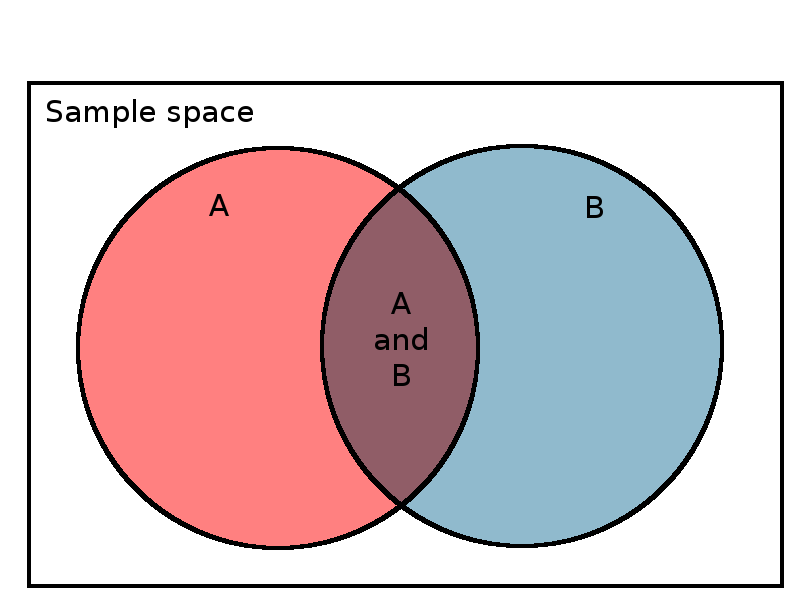
\includegraphics[width=3in]{../images/ch4_venn_ovr}\par
}
\end{frame}

%%%%%%%%%%
\begin{frame}{Venn diagrams, disjoint events}
\begin{block}{}
\large Disjoint events are represented non-overlapping circles.
\end{block}
{\centering
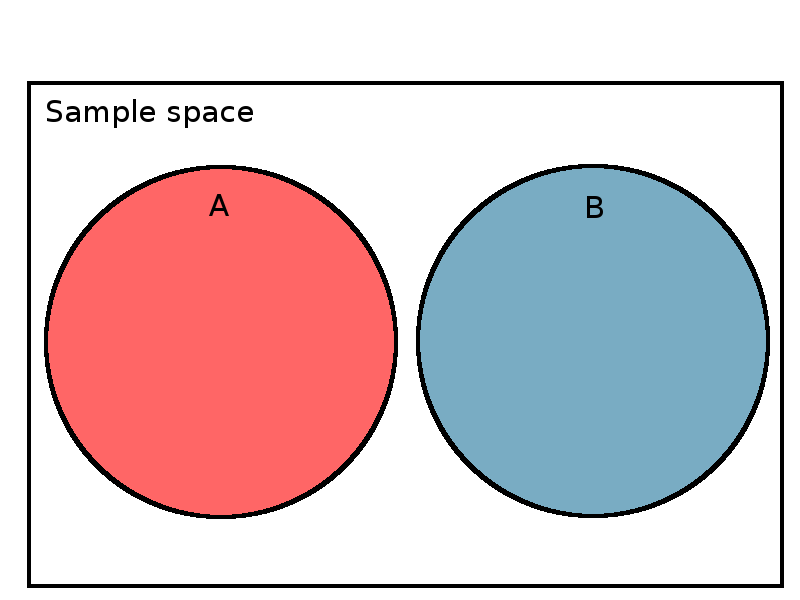
\includegraphics[width=3in]{../images/ch4_venn_dsj}\par
}
\end{frame}

%%%%%%%%%%
\begin{frame}{Venn diagrams, complements}
\begin{block}{}
\large Complements are the whole sample space except the event area.
\end{block}
{\centering
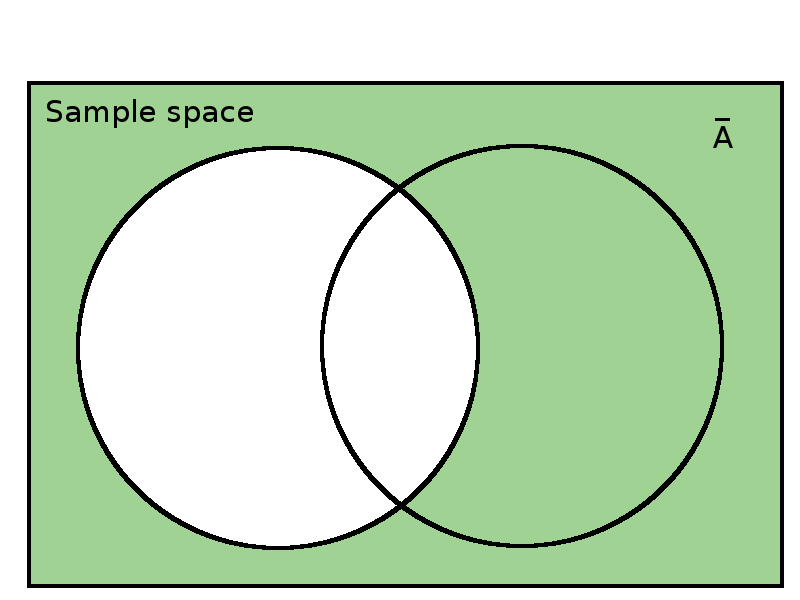
\includegraphics[width=3in]{../images/ch4_venn_a_comp}\par
}
\end{frame}

%%%%%%%%%%
\begin{frame}{Addition rule}
\begin{block}{}
The general rule for calculating probabilities of compound events is to count the outcomes satisfying A and the outcomes satisfying B, making sure to only count each outcome once, and then divide by total number of outcomes.
\end{block}

\pause
\begin{block}{}
\begin{itemize}
\item The formal rule is\\
\smallskip\eq{P(A \text{ or } B) = P(A) + P(B) - P(A \text{ and } B)}
\medskip Note: $P(A \text{ and } B)$ is the joint probability of $A$ and $B$.

\pause\medskip
\item For disjoint events, $P(A \text{ and } B) = 0$, so the rule becomes,\\
\smallskip\eq{P(A \text{ or } B) = P(A) + P(B)}
\end{itemize}
\end{block}
\end{frame}

%%%%%%%%%%
\begin{frame}{Addition rule, example}
\begin{block}{}
Suppose a statistics class has 100 students. On the midterm, 40 students got an A (event $A$) and 30 students got a B (event $B$).
\end{block}

{\centering
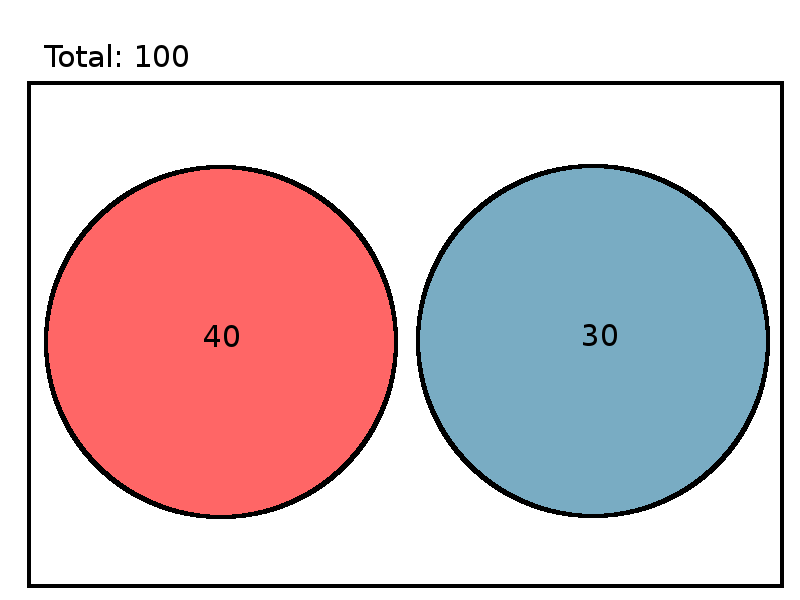
\includegraphics[width=3in]{../images/ch4_venn_dsj_ex}\par
}
\end{frame}

%%%%%%%%%%
\begin{frame}{Addition rule, example cont.}
\begin{block}{}
Suppose a statistics class has 100 students. On the midterm, 40 students got an A (event $A$) and 30 students got a B (event $B$).
\end{block}

\begin{exampleblock}{}
What is the probability that a randomly selected student got an A or a B?
\begin{itemize}
\pause
\item By the general rule, 40 outcomes for event $A$ and 30 outcomes for event $B$, and none are counted twice. So,\\
\smallskip\eq{P(A \text{ or } B) = \frac {40 + 30}{100} = 0.7}
\pause
\item By the formal rule, $P(A \text{ or } B) = P(A) + P(B) - P(A \text{ and } B)$,\\
\smallskip\eq{P(A) = 0.4 \qquad P(B) = 0.3 \qquad P(A \text{ and } B) = 0}
\smallskip\eq{P(A \text{ or } B) = 0.4 + 0.3 - 0 = 0.7}
\end{itemize}
\end{exampleblock}
\end{frame}

%%%%%%%%%%
\begin{frame}{Addition rule, example 2}
\begin{block}{}
Suppose a statistics class has 100 students. On the midterm, 40 students got an A (event $A$),  70 students are female (event $B$) and 25 of the female students got an A.
\end{block}

{\centering
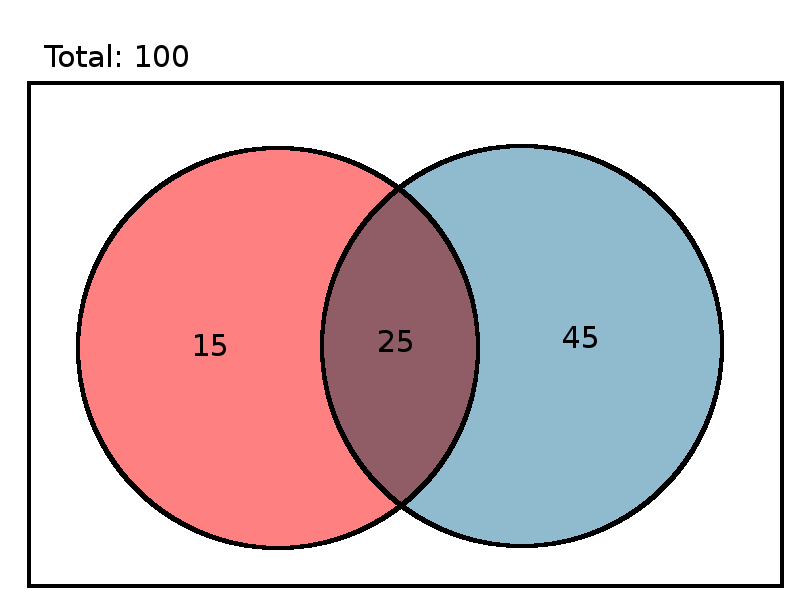
\includegraphics[width=3in]{../images/ch4_venn_ovr_ex}\par
}
\end{frame}

%%%%%%%%%%
\begin{frame}{Addition rule, example 2 cont.}
\begin{block}{}
Suppose a statistics class has 100 students. On the midterm, 40 students got an A (event $A$),  70 students are female (event $B$) and 25 of the female students got an A.
\end{block}
\begin{exampleblock}{}
What is the probability that a randomly selected student got an A or is female?
\begin{itemize}
\pause
\item By the general rule, if outcomes were counted as in the previous example,\\
\smallskip\eq{P(A \text{ or } B) \ne \frac {40 + 70}{100} = 1.1}

\pause
\item The females who got A's were counted twice. Instead, count distinct outcomes in the circles of the Venn diagram.\\
\smallskip\eq{P(A \text{ or } B) = \frac {15 + 25 + 45}{100} = 0.85}

\end{itemize}
\end{exampleblock}

\end{frame}

%%%%%%%%%%
\begin{frame}{Addition rule, example 2 cont.}
\begin{block}{}
Suppose a statistics class has 100 students. On the midterm, 40 students got an A (event $A$),  70 students are female (event $B$) and 25 of the female students got an A.
\end{block}

\begin{exampleblock}{}
What is the probability that a randomly selected student got an A or is female?
\begin{itemize}
\pause
\item By the formal rule, $P(A \text{ or } B) = P(A) + P(B) - P(A \text{ and } B)$,\\
\smallskip\eq{P(A) = 0.4 \qquad P(B) = 0.7 \qquad P(A \text{ and } B) = 0.25}
\smallskip\eq{P(A \text{ or } B) = 0.4 + 0.7 - 0.25 = 0.85}
\end{itemize}
\end{exampleblock}
\end{frame}

%%%%%%%%%%
\begin{frame}{Addition rule, example 2 table}
\begin{block}{}
Suppose a statistics class has 100 students. On the midterm, 40 students got an A (event $A$),  70 students are female (event $B$) and 25 of the female students got an A.
\end{block}

\begin{exampleblock}{}
Construct a contingency table for this situation.\\
\pause
\medskip
{\centering
\begin{tabular}{c | c  c | c}
\multicolumn{1}{c}{} & \multicolumn{2}{c}{Midterm grade}\\
Gender & A & Not A & Total\\
\hline
Female & 25 & \onslide<4->{45} & 70\\
Male & \onslide<4->{15} & \onslide<5->{15} & \onslide<3->{30} \\
\hline
Total & 40 & \onslide<3->{60} & 100
\end{tabular}\par
}
\end{exampleblock}
\end{frame}

%%%%%%%%%%
\begin{frame}{Complements, revisited}
\begin{block}{}
\begin{itemize}
\item Recall, an event and its complement comprise the whole sample space. Whatever the result of a trial, it satisfies either the event or its complement.\\
\smallskip\eq{P(A \text{ or } \bar A) = 1}
\pause
\item Also, complements are disjoint, so the addition rule is\\
\smallskip\eq{P(A \text{ or } \bar A) = P(A) + P(\bar A)}
\pause
\item Then,\\
\smallskip\eq{P(A) + P(\bar A) = 1}
\smallskip\eq{P(A) = 1 -  P(\bar A)}
\smallskip\eq{P(\bar A) = 1 - P(A)}
\end{itemize}

\end{block}
\end{frame}

%%%%%%%%%%
\begin{frame}{Practice: Cancer screening}
\begin{block}{}
{\centering
\begin{tabular}{c | c  c | c}
\multicolumn{1}{c}{} & \multicolumn{2}{c}{Test Result}\\
Diagnosis & Positive & Negative & Total \\
\hline
Cancer & 74 & 13 & 87\\
No cancer & 26 & 887 & 913\\
\hline
Total & 100 & 900 & 1000
\end{tabular}\par
}
\end{block}

\begin{exampleblock}{}
What is the probability of a randomly selected person having cancer ($A$) or not having cancer ($B$)?

\begin{itemize}
\pause
\item Having cancer and not having cancer are complements,\\
\smallskip\eq{ P(A \text{ or } B) = 1 }
\end{itemize}
\end{exampleblock}
\end{frame}

%%%%%%%%%%
\begin{frame}{Practice: Cancer screening, cont.}
\begin{block}{}
{\centering
\begin{tabular}{c | c  c | c}
\multicolumn{1}{c}{} & \multicolumn{2}{c}{Test Result}\\
Diagnosis & Positive & Negative & Total \\
\hline
Cancer & 74 (0.074) & 13 (0.013) & 87 (0.087)\\
No cancer & 26 (0.026) & 887 (0.887) & 913 (0.913)\\
\hline
Total & 100 (0.1) & 900 (0.9) & 1000 (1)
\end{tabular}\par
}
\end{block}

\begin{exampleblock}{}
What is the probability of a randomly selected person having cancer ($A$) or getting a positive test result ($B$)?

\begin{itemize}
\pause
\item Using the addition rule,\\
\smallskip\eq{ P(A \text{ or } B) = P(A) + P(B) - P(A \text{ and } B)}
\pause\eq{ = 0.087 + 0.1 - 0.074 = 0.113}
\end{itemize}
\end{exampleblock}
\end{frame}

%%%%%%%%%%
\begin{frame}{Practice: Cancer screening, cont.}
\begin{block}{}
{\centering
\begin{tabular}{c | c  c | c}
\multicolumn{1}{c}{} & \multicolumn{2}{c}{Test Result}\\
Diagnosis & Positive & Negative & Total \\
\hline
Cancer & 74 (0.074) & 13 (0.013) & 87 (0.087)\\
No cancer & 26 (0.026) & 887 (0.887) & 913 (0.913)\\
\hline
Total & 100 (0.1) & 900 (0.9) & 1000 (1)
\end{tabular}\par
}
\end{block}

\begin{exampleblock}{}
What is the probability of a test being wrong? That is, what is the probability of getting a false positive ($A$) or a false negative ($B$)?

\begin{itemize}
\pause
\item The events are disjoint. Using simplified addition rule,\\
\smallskip\eq{ P(A \text{ or } B) = P(A) + P(B) }
\pause\eq{ = 0.026 + 0.013 = 0.039}
\end{itemize}
\end{exampleblock}
\end{frame}

%%%%%%%%%%
\begin{frame}<handout:0>{Group work}
\begin{block}{}
\large
\begin{itemize}
\item For questions 1 through 3, complete part (b).
\item Probabilities can be expressed as fractions.
\end{itemize}
\end{block}
\end{frame}

%
% Section 2.3
%
\subsection{Multiplication Rule}

%%%%%%%%%%
\begin{frame}{Independent events}
\begin{block}{}
Two events are said to be \bt{independent} if the probability of one is unaffected by the occurrence of the other.
\end{block}

\pause

\begin{exampleblock}{Example}
\begin{itemize}
\item Let $A$ = get a head on the first flip\\
and $B$ = get a tail on the second flip.\\
$P(B) = \frac 1 2$ regardless of what happens on the first flip.
\end{itemize}
\end{exampleblock}
\end{frame}

%%%%%%%%%%
\begin{frame}{Dependent events}
\begin{block}{}
If two events are not independent, then they are \bt{dependent}. That is, the probability of one changes depending on the outcome of the other.
\end{block}
\end{frame}

%%%%%%%%%%
\begin{frame}{Dependent events, examples}

\begin{exampleblock}{Example}
Consider an urn with 2 red balls and 3 blue balls. A trial consists of randomly selecting a ball from the urn and not replacing it.\\
\pause
\medskip Let $A$ = get a red ball the first trial\\
 and $B$ = get a blue ball the second trial.
\begin{itemize}
\pause
\item If $A$ occurs, then $P(B) = 3 / 4$
\pause
\item If $A$ does not occur, then $P(B) =  2 / 4$
\end{itemize}
\end{exampleblock}

\pause

\begin{exampleblock}{Example}
The probability of a randomly selected student getting an A on the final is probably different depending on whether they got an A on the midterm.
\end{exampleblock}
\end{frame}


%%%%%%%%%%
\begin{frame}{Dependent events as independent}
\begin{block}{}
When dealing with large populations and small sample sizes, events that are technically dependent can be treated as independent. The rule of thumb we will use is sample sizes less than 5\% of population can be treated as independent.
\end{block}

\pause
\begin{exampleblock}{Example}
Suppose the urn has 2000 red balls and 3000 blue balls. The probability of selecting a blue ball is very close to $3/5$, regardless of whether a red ball was previously selected or not.
\end{exampleblock}
\end{frame}

%%%%%%%%%%
\begin{frame}{Conditional probability}
\begin{block}{}
The \bt{conditional probability} of an event is the probability assuming another event occurred. 
\begin{itemize}
\pause
\item It is denoted $P(B|A)$ and read as ``probability of $B$ given $A$"
\pause
\item For independent events, $P(B|A) = P(B)$
\end{itemize}
\end{block}

\pause
\begin{exampleblock}{Example}
There is an urn with 2 red balls and three blue balls. A trial consists of randomly selecting a ball from the urn and not replacing it.\\
\medskip Let $A$ = get a red ball the first trial\\
 and $B$ = get a blue ball the second trial.
\begin{itemize}
\pause
\item $P(B | A) = 3 / 4$
\pause
\item $P(B | \bar A) =  2 / 4$
\end{itemize}

\end{exampleblock}
\end{frame}

%%%%%%%%%%
\begin{frame}{Multiplication rule}
\begin{block}{}
To find the probability of all events in a series of trials, multiply the probability of the first by the probability of the second given the first occurred, etc.\\
\medskip
\pause
Formally,\\ \smallskip
\eq{P(A \text{ and } B) = P(A) \times P(B|A)}
\pause\medskip
For independent events,\\ \smallskip
\eq{P(A \text{ and } B) = P(A) \times P(B)}
\end{block}
\end{frame}

%%%%%%%%%%
\begin{frame}{Multiplication rule, example}
\begin{exampleblock}{Example}
There is an urn with 2 red balls and 3 blue balls. A trial consists of randomly selecting a ball from the urn and not replacing it.\\
\medskip 
What is the probability of selecting a red ball and then selecting a blue ball?
\begin{itemize}
\pause
\item Let $A$ = get a red ball the first trial\\
 and $B$ = get a blue ball the second trial.\\

\pause
\item $B$ is dependent on $A$.\\ \smallskip
\eq{P(A \text{ and } B) = P(A) \times P(B|A)} \smallskip

\pause
\item $P(A) = 2/5 \qquad P(B|A) = 3/4$\\ \smallskip

\pause
\eq{P(A \text{ and } B) = \frac 2 5 \times \frac 3 4 = \frac 6 {20} = \frac 3 {10} = 0.3}

\end{itemize}

\end{exampleblock}
\end{frame}

%%%%%%%%%%
\begin{frame}{Multiplication rule, example}
\begin{exampleblock}{Example}
Consider flipping a coin three times.\\
\medskip 
What is the probability of get heads on the first two flips and a tail on the third (HHT)?
\begin{itemize}
\pause
\item Let $A$ = get a head the first flip,\\
 $B$ = get a head on the second flip,\\
and $C$ = get a tail on the third flip.

\pause
\item $A$, $B$ and $C$ are independent events.\\ \smallskip
\eq{P(A \text{ and } B \text{ and } C) = P(A) \times P(B) \times P(C)} \smallskip

\pause
\item $P(A) = P(B) = P(C) = 1/2$\\ \smallskip

\pause
\eq{P(A \text{ and } B \text{ and } C) = \frac 1 2 \times \frac 1 2 \times \frac 1 2 = \frac 1 8}

\end{itemize}

\end{exampleblock}
\end{frame}

%%%%%%%%%%
\begin{frame}{Tree diagrams}
\begin{block}{}
\bt{Tree diagrams} are a good way to visualize events in a series of trials.
\end{block}
\bigskip
{\centering
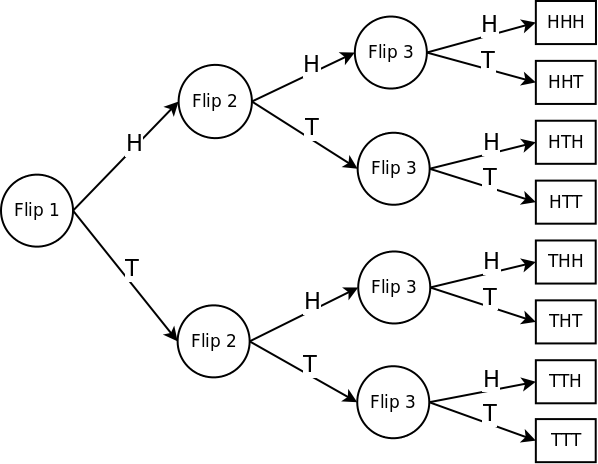
\includegraphics[width=3in]{../images/tree_diagram_coin}\par
}
\end{frame}

%%%%%%%%%%
\begin{frame}{Tree diagram, urn example}

{\centering
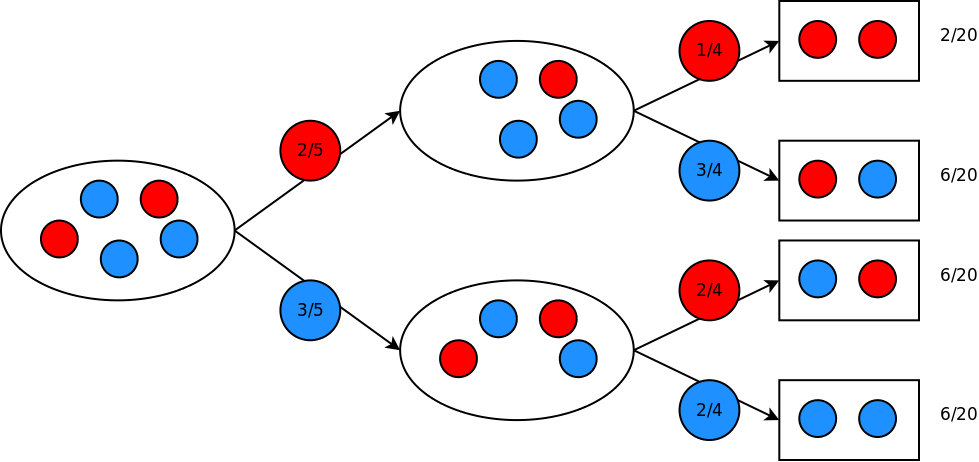
\includegraphics[width=4in]{../images/tree_diagram_balls}\par
}
\end{frame}

%%%%%%%%%%
\begin{frame}{Practice: Cancer screening}
\begin{block}{}
{\centering
\begin{tabular}{c | c  c | c}
\multicolumn{1}{c}{} & \multicolumn{2}{c}{Test Result}\\
Diagnosis & Positive & Negative & Total \\
\hline
Cancer & 74 & 13 & 87\\
No cancer & 26 & 887 & 913\\
\hline
Total & 100 & 900 & 1000
\end{tabular}\par
}
\end{block}

\begin{exampleblock}{}
What is the probability of two randomly selected people both having positive test results?

\begin{itemize}
\pause
\item Sample size of 2 is less than 5\% of population of 1000, so can treat events as independent.
\pause
\item $P(\text{one is positive}) = \frac {100}{1000} = 0.1$
\pause
\item $P(\text{both positive}) = 0.1 \times 0.1 = 0.01$
\end{itemize}
\end{exampleblock}

\end{frame}

%%%%%%%%%%
\begin{frame}{Practice: Statistics club}
\begin{block}{}
The Metro State Statistics Club has 10 members, 6 men and 4 women. They need to select a president, a vice-president and a treasurer. They decide to choose members randomly for the officers positions, in order.
\end{block}
\end{frame}

%%%%%%%%%%
\begin{frame}{Practice: Statistics club, cont.}
\begin{exampleblock}{}
What is the probability that women are selected for president and vice-president, and a man for treasurer?
\begin{itemize}
\pause
\item $A$ = Woman selected president\\
$B$ = Woman selected vice-president\\
$C$ = Man selected treasurer
\pause
\item $P(A \text{ and } B \text{ and } C) = P(A) \times P(B|A) \times P(C | A \text{ and } B)$\\
\pause
\item $P(A) = \frac 4{10} = 0.4$\\
$P(B|A) = \frac 3 9 = 0.33$\\
$P(C | A \text{ and } B) = \frac 6 8 = .75$

\pause
\item $P(A \text{ and } B \text{ and } C) = 0.4 \times 0.33 \times 0.75 = 0.099$ 
\end{itemize}
\end{exampleblock}
\end{frame}

%%%%%%%%%%
\begin{frame}{Recap of probability rules}
\begin{block}{}
\begin{itemize}
\item To calculate the probability of at least one of two events occurring ($A$ \bt{or} $B$), use the addition rule. Be aware of whether the events are disjoint or not.

\pause
\item To calculate  the probability of all of a sequence of two, or more, events occurring ($A$ \bt{and} $B$), use the multiplication rule. Be aware of whether the events are independent or dependent.
\end{itemize}
\end{block}
\end{frame}

%%%%%%%%%%
\begin{frame}{Testing for independence}
\begin{block}{}
It is sometimes difficult to tell if events are independent. The rule for independent events, that $P(B|A) = P(B)$, can be used to test for independence.
\end{block}
\end{frame}

%%%%%%%%%%
\begin{frame}{Testing for independence, example}
\begin{exampleblock}{Example}
Consider rolling two fair six-sided dice. Let $A$ = total of the dice is 5 and $B$ = at least one of the dice is a 3.\\
\medskip
Are $A$ and $B$ independent events?
\begin{itemize}
\pause
\item $P(B) = P(\text{first die is 3 or second die is 3}) $\\
$P(B) = P(\text{first die is 3}) + P(\text{second die is 3}) - P(\text{both are 3}) $\\
$P(B) = \frac 1 6 + \frac 1 6 - \frac 1 {36} = \frac {11}{36}$
\pause
\item If $A$ occurred, then the possible dice values are\\ \smallskip
\eq{\set{(1,4), (2,3), (3,2), (4,1)}} \smallskip

\pause
\item $P(B|A) = \frac 2 4 = \frac 1 2$

\pause
\item $P(B) \ne P(B \mid A)$\ldots $A$ and $B$ are not independent.
\end{itemize} 
\end{exampleblock}
\end{frame}

%%%%%%%%%%
\begin{frame}<handout:0>{Group work}
\begin{block}{}
\large
\begin{itemize}
\item For questions 1 through 3, complete part (c).
\item Probabilities can be expressed as fractions.
\end{itemize}
\end{block}
\end{frame}


\end{document}